\documentclass{standalone}

\usepackage{tikz}
\usetikzlibrary{positioning}
\usetikzlibrary{arrows.meta}
\usepackage{physics}

\begin{document}

\resizebox{700px}{!}{%
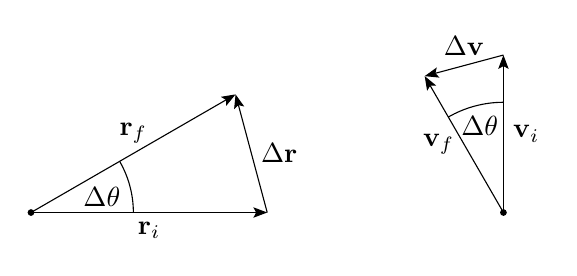
\begin{tikzpicture}
    [
	arrow/.style={arrows = {-Stealth[length=5pt, inset=1pt]}}
    ]

    % radius vectors
    \draw[fill=black] (0, 0) circle (1pt);

    \draw[arrow] (0, 0) -- (3, 0)
	node [midway, below] {$\vb{r}_i$}
	coordinate (ri) [right];
    \draw[arrow, rotate=30] (0, 0) -- (3, 0)
	node [midway, above] {$\vb{r}_f$}
	coordinate (rf) [right];
    \draw[arrow] (ri) -- (rf)
	node [midway, right] {$\Delta \vb{r}$};

    \draw[draw=black] (1.3, 0) arc (0:30:1.3);
    \node at (0.9, 0.2) {$\Delta \theta$};

    % velocity vectors
    \draw[fill=black] (6, 0) circle (1pt);

    \draw[arrow] (6, 0) -- (6, 2)
	node [midway, right] {$\mathbf{v}_i$}
	coordinate (vi) [above];
    \draw[arrow, rotate around={30:(6, 0)}] (6, 0) -- (6, 2)
	node [midway, left] {$\mathbf{v}_f$}
	coordinate (vf) [above];
    \draw[arrow] (vi) -- (vf)
	node [midway, above] {$\Delta \vb{v}$};

    \draw[draw=black] (6, 1.4) arc (90:120:1.4);
    \node at (5.7, 1.1) {$\Delta \theta$};

\end{tikzpicture}
}

\end{document}
